\documentclass[titlepage,a4paper,12pt]{report}
\usepackage{amssymb,amsfonts,amsmath}
\usepackage{fullpage}
\usepackage{graphicx}
%\usepackage[cc]{titlepic}
\usepackage{amsthm}
\newtheorem{definition}{Definition}[section]
\newtheorem{example}{Example}[section]
\newtheorem{theorem}{Theorem}[section]
\newtheorem{exercise}{Exercise}[section]
\newtheorem{corollary}{Corollary}[section]
\newtheorem{proposition}{Proposition}[section]
\pdfpagewidth 8.5in
\pdfpageheight 11in
\setlength\topmargin{-0.5in}
\setlength\headheight{0in}
\setlength\headsep{0in}
\setlength\textheight{9.5in}
\setlength\textwidth{7.0in}
\setlength\oddsidemargin{-0.5in}
\setlength\evensidemargin{1.0in}
\setlength\parindent{0.25in}
\setlength\parskip{0.25in}
%\begin{titlepage}
%\usepackage{titlepic}
%\titlepic{
\includegraphics[width=0.2\textwidth]{uz1.png}}
%
%\title{\textbf{HMTH111 Calculus 2}}
%\author{Nhawu. G\\
%		Department of Mathematics\\
%		University of Zimbabwe, ZIM}
%
%\end{titlepage}

\begin{document}
\begin{titlepage}
 
\begin{center}
 
 
% Upper part of the page

\includegraphics[width=0.15\textwidth]{uz1.png}\\[1cm]
 
\textsc{\LARGE University of Zimbabwe}\\[1.5cm]
 
\textsc{\Large HMTHCS111 CALCULUS 2}\\[0.5cm]
 
 
% Title

{ \huge \bfseries Calculus of Several Variables}\\[0.4cm]
 

 
% Author and supervisor
\begin{minipage}{0.4\textwidth}
\begin{center} \large
\emph{Author:}\\
G. \textsc{Nhawu}
\end{center}
\end{minipage}
\begin{minipage}{0.4\textwidth}
\begin{flushright} \large
\emph{Department:} \\
\textsc{Mathematics and Computational Sciences}
\end{flushright}
\end{minipage}

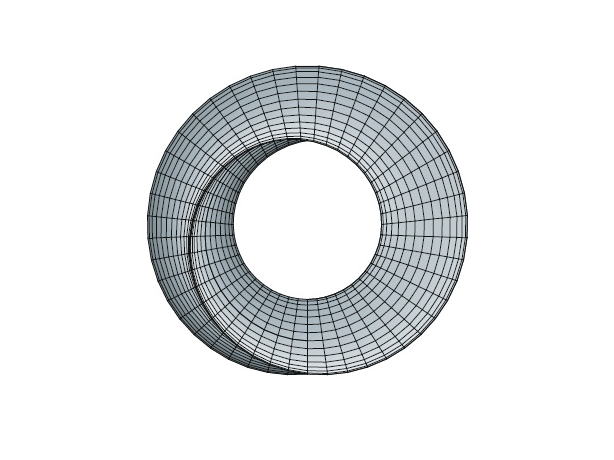
\includegraphics[width=0.7\textwidth]{umblictorus.png}\\[1cm]
 \vfill
 
 
% Bottom of the page
{\large \today}
 
\end{center}
 
\end{titlepage}
%\maketitle
\tableofcontents
\setcounter{chapter}{4}
\chapter{Vector-Valued Functions}
\begin{center}
\small{\parbox{18cm}{
		\begin{raggedright}
		{\small
		\textit{If you think dogs can't count, try putting three dog biscuits in your pocket and then giving Fido only two of them.}
 }
 
				\vspace{.5cm}\hfill{---Phil Pastoret}
		\end{raggedright}
	}
} 
\end{center}
This chapter introduces the concept of vector-valued functions. Vector-valued functions can be used to study curves in the plane and in space. These functions can  also be used to study the motion of an object along a curve.
\section{Plane Curves and Parametric Equations}
Until now, we have been representing a graph by a single equation involving two variables. Consider the path followed by an object that is propelled into the air at an angle of $45^\circ$. If the initial velocity of the object is $48$ meters per second, the object travels the parabolic path given by 
\[y=-\dfrac{x^2}{72}+x, \quad \mbox{Rectangular form}.\]
However, this equation does not tell the whole story. Although it does tell you where the object has been, it doesn't tell you when the object was at a given point $(x,y)$. To determine this time, you introduce a third variable $t$, called a \textbf{parameter}. By writing both $x$ and $y$ as functions of $t$, you obtain the \textbf{parametric equations}
\[x=24\sqrt{2}t \quad {\mbox{and}} \quad y=-16t^2+24\sqrt{2}t \quad {\mbox{Parametric equations}}. \]
From this set of equations, you can determine that at time $t=0$, the object is at the point $(0,0)$. Similarly, at time $t=1$, the object is at the point $(24\sqrt{2}, 24\sqrt{2}-16)$, and so on.
\begin{theorem}
If $f$ and $g$ are continuous functions of $t$ on an interval $I$, then the equations 
\[x=f(t) \quad \mbox{and} \quad y=g(t)\] are called \textbf{parametric equations} and $t$ is called a \textbf{parameter}. 
\end{theorem}
\noindent A \textbf{space curve} is the set of all ordered triples $(f(t), g(t), h(t))$ together with their defining parametric equations
\[x=f(t), \quad y=g(t) \quad \mbox{and} \quad z=h(t)\] where $f,g$ and $h$ are continuous functions of $t$ on the interval $I$.
\begin{theorem}
A function of the form 
\[{\bf{r}}(t) = f(t){\bf{i}}+g(t){\bf{j}} \quad \mbox{Plane}\] or \[{\bf{r}}(t)=f(t){\bf{i}}+g(t){\bf{j}}+h(t){\bf{k}} \quad \mbox{Space} \] is a \textbf{vector-valued function}, where the \textbf{component functions} $f,g$ and $h$ are real-valued functions of the parameter $t$. Vector-valued functions are sometimes denoted as ${\bf{r}}(t)=(f(t), g(t))$ or ${\bf{r}}(t)=(f(t, g(t), h(t))$.
\end{theorem}
\noindent Vector-valued functions serve dual roles in the representation of curves. By letting the parameter $t$ represent time, we can use a vector-valued function to represent \textit{motion} along a curve. Or, in the more general case, we can use a vector-valued function to \textit{trace the graph} of a curve. 
\begin{figure}
\input{curve.pic}
\caption{Curve in plane}
\end{figure}
\noindent Unless stated otherwise, the \textbf{domain} of a vector-valued function ${\bf{r}}$ is considered to be the intersection of the domains of the component functions $f,g$ and $h$. For example, the domain of \\${\bf{r}}(t)=\ln t {\bf{i}}+\sqrt{1-t}{\bf{j}}+t{\bf{k}}$ is the interval $(0,1]$.
\section{Limits and Continuity}
Many techniques and definitions used in calculus of real-valued functions can be applied to vector-valued functions. For example, we can add and subtract vector-valued functions, multiply a vector-valued function with a scalar, take the limit of a vector-valued function, differentiate a vector-valued function, and so on.
\begin{eqnarray*}
{\bf{r}}_1(t) + {\bf{r}}_2(t) &=& [f_1(t){\bf{i}}+g_1(t){\bf{j}}] +[f_2(t){\bf{i}}+g_2(t){\bf{j}}] \\
&=& [f_1(t)+f_2(t)] {\bf{i}} + [g_1(t)+g_2(t)] {\bf{j}}.
\end{eqnarray*}
\section{Definition of the Limit of a Vector-Valued Function }
If ${\bf{r}}$ is a vector-valued function such that ${\bf{r}}(t) = f(t){\bf{i}}+g(t){\bf{j}}$, then 
\[\lim _{t\rightarrow a} {{\bf{r}}(t)} =\left[ \lim _{t\rightarrow a}{f(t)}\right]{\bf{i}} +\left[ \lim _{t\rightarrow a}{g(t)}\right]{\bf{j}} \quad \quad \mbox{Plane}\] provided $f$ and $g$ have limits as $t\rightarrow a$.

\noindent If ${\bf{r}}$ is a vector-valued function such that ${\bf{r}}(t)=f(t){\bf{i}}+g(t){\bf{j}}+h(t){\bf{k}}$, then 
\[\lim _{t\rightarrow a} {{\bf{r}}(t)} =\left[ \lim _{t\rightarrow a}{f(t)}\right]{\bf{i}} +\left[ \lim _{t\rightarrow a}{g(t)}\right]{\bf{j}} +\left[ \lim _{t\rightarrow a}{h(t)}\right]{\bf{k}} \quad \quad \mbox{Space}\] provided $f,g$ and $h$ have limits as $t\rightarrow a$.

\noindent If ${\bf{r}}(t)$ approaches the vector ${\bf{L}}$ as $t\rightarrow a$, the length of the vector ${\bf{r}}(t)-{\bf{L}}$ approaches $0$, that is 
 \[|{\bf{r}}(t)-{\bf{L}}|\rightarrow 0 \quad  \mbox{as} \quad t\rightarrow a.\]
 
\noindent The next theorem extends the notion of continuity of vector-valued functions.
\begin{theorem}
A vector-valued function ${\bf{r}}$ is \textbf{continuous at a point} given by $t=a$ if the limit of ${\bf{r}}(t)$ exists as $t\rightarrow a$ and 
\[\lim _{t\rightarrow a} {\bf{r}}(t)={\bf{r}}(a).\]
\end{theorem}
\noindent A vector-valued function ${\bf{r}}$ is \textbf{continuous on an interval $I$} if it is continuous at every point in the interval. It follows that a vector-valued function is continuous at $t=a$ if and only if each of its component functions is continuous at $t=a$.

\begin{example}
Discuss the continuity of the vector-valued function given by 
\[{\bf{r}}(t)=t{\bf{i}}+a{\bf{j}}+(a^2-t^2){\bf{k}}\] at $t=0$.

\noindent \textbf{Solution:} As $t$ approaches $0$, the limit is 
\begin{eqnarray*}
\lim _{t\rightarrow 0} {\bf{r}}(t) &=& \left[ \lim _{t\rightarrow 0}{t}\right]{\bf{i}} +\left[ \lim _{t\rightarrow 0}{a}\right]{\bf{j}}+\left[ \lim _{t\rightarrow 0}{(a^2-t^2)}\right]{\bf{k}}\\
&=& 0{\bf{i}}+a{\bf{j}}+a^2{\bf{k}}\\
&=& a{\bf{j}}+a^2{\bf{k}}.
\end{eqnarray*}
Because 
\begin{eqnarray*}
{\bf{r}}(0) &=& (0){\bf{i}} +(a){\bf{j}} +(a^2){\bf{k}}\\
&=& a{\bf{j}}+a^2{\bf{k}}.
\end{eqnarray*}
We can conclude that ${\bf{r}}$ is continuous at $t=0$.
\end{example}
\section{Differentiation and Integration of Vector-Valued Functions}
\subsection{Differentiation of Vector-Valued Functions}
The definition of the derivative of a vector-valued function parallels the definition given for real-valued functions.
\begin{theorem}
The \textbf{derivative of a vector-valued function ${\bf{r}}$} is defined by 
\[{\bf{r}}'(t)=\lim _{\bigtriangleup t \rightarrow 0}\dfrac{{\bf{r}}(t+\bigtriangleup t)-{\bf{r}}(t)}{\bigtriangleup t }\] for all $t$ for which the limit exists. If ${\bf{r}}'(t)$ exists, then ${\bf{r}}$ is \textbf{differentiable at t}. In addition to ${\bf{r}}'(t)$, other notations for the derivative of a vector-valued function are 
\[D_t[{\bf{r}}(t)], \quad \dfrac{d}{dt}[{\bf{r}}(t)] \quad \mbox{and} \quad \dfrac{d{\bf{r}}}{dt}.\]
\end{theorem}
\noindent Differentiation of vector-valued functions can be done on a \textit{component-by-component basis}. To see why this is true, consider the function given by
\[{\bf{r}}(t)=f(t){\bf{i}}+g(t){\bf{j}}.\]
Applying the definition of the derivative produces the following 
\begin{eqnarray*}
{\bf{r}}'(t) &=& \lim _{\bigtriangleup t \rightarrow 0}\dfrac{{\bf{r}}(t+\bigtriangleup t)-{\bf{r}}(t)}{\bigtriangleup t }\\
&=& \lim _{\bigtriangleup t \rightarrow 0} \dfrac{f(t+\bigtriangleup t){\bf{i}}+g(t+\bigtriangleup t){\bf{j}}-f(t){\bf{i}}-g(t){\bf{j}}}{\bigtriangleup t}\\
&=& \lim _{\bigtriangleup t \rightarrow 0} \left \{ \left[ \dfrac{f(t+\bigtriangleup t)-f(t)}{\bigtriangleup t}\right]{\bf{i}}+\left[\dfrac{g(t+\bigtriangleup t)-g(t)}{\bigtriangleup t}\right]{\bf{j}}\right \}\\
&=& \left \{\lim _{\bigtriangleup t\rightarrow 0} \left[ \dfrac{f(t+\bigtriangleup t)-f(t)}{\bigtriangleup t}\right]{\bf{i}}\right \}+\left \{\lim _{\bigtriangleup t\rightarrow 0}\left[\dfrac{g(t+\bigtriangleup t)-g(t)}{\bigtriangleup t}\right]{\bf{j}}\right \}\\
&=& f'(t){\bf{i}}+g'(t){\bf{j}}.
\end{eqnarray*}
Note that the derivative of the vector-valued function ${\bf{r}}$ is itself a vector-valued function. ${\bf{r}}'(t)$ is a vector tangent to the curve given by ${\bf{r}}(t)$ and pointing in the direction of increasing  $t$-values.
\begin{theorem}
If ${\bf{r}}(t)=f(t){\bf{i}}+g(t){\bf{j}}$, where $f$ and $g$ are differentiable functions of $t$, then 
\[{\bf{r}}'(t)=f'(t){\bf{i}}+g'(t){\bf{j}}.\]
If ${\bf{r}}(t)=f(t){\bf{i}}+g(t){\bf{j}}+h(t){\bf{k}}$, where $f,g$ and $h$ are differentiable functions of $t$, then 
\[{\bf{r}}'(t)=f'(t){\bf{i}}+g'(t){\bf{j}}+h'(t){\bf{k}}.\]
\end{theorem}
\begin{example}
For the vector-valued function given by ${\bf{r}}(t)=t{\bf{i}}+(t^2+2){\bf{j}}$, find ${\bf{r}}'(t)$.

\noindent \textbf{Solution:} ${\bf{r}}'(t)={\bf{i}}+2t{\bf{j}}$.
\end{example}
\noindent Higher-order derivatives of vector-valued functions are obtained by successive differentiation of each component function.
\begin{example}
For the vector-valued function given by ${\bf{r}}(t)=\cos t{\bf{i}}+\sin t {\bf{j}}+2t{\bf{k}}$, find each of the following (i)\, ${\bf{r}}'(t)$ \quad (ii)\, ${\bf {r}}''(t)$ \quad (iii)\, ${\bf{r}}'(t) \cdot {\bf {r}}''(t) $ \quad (iv)\, ${\bf{r}}'(t) \times {\bf {r}}''(t) $.

\noindent \textbf{Solution:} (i)\, ${\bf{r}}'(t)=-\sin t {\bf{i}}+\cos t {\bf{j}} +2{\bf{k}}$.\\
(ii)\, ${\bf{r}}''(t)=-\cos t {\bf{i}}-\sin  t {\bf{j}} +0{\bf{k}}=-\cos t {\bf{i}}-\sin  t {\bf{j}}$.\\
(iii)\, ${\bf{r}}'(t) \cdot {\bf {r}}''(t) =\sin t \cos t-\sin t \cos t =0 $.\\
(iv)\, ${\bf{r}}'(t) \times {\bf {r}}''(t) =\begin{vmatrix}
{\bf{i}} & {\bf{j}} & {\bf{k}} \\
-\sin t & \cos t & 2 \\
-\cos t & -\sin t & 0
\end{vmatrix} =\begin{vmatrix}
\cos t & 2 \\
-\sin t & 0
\end{vmatrix} {\bf{i}}-\begin{vmatrix}
-\sin t & 2 \\
-\cos t & 0
\end{vmatrix} {\bf{j}} +\begin{vmatrix}
-\sin t & \cos t \\
-\cos t & -\sin t
\end{vmatrix} {\bf{k}} \\ =2\sin t {\bf{i}}-2\cos t {\bf{j}} +{\bf{k}}$. 
\end{example}
\noindent The parametrization of the curve represented by the vector-valued function 
\[{\bf{r}}(t)=f(t){\bf{i}}+g(t){\bf{j}}+h(t){\bf{k}}\] is \textbf{smooth on an open interval I} if $f', g'$ and $h'$ are continuous on $I$ and ${\bf{r}}'(t)\neq 0$ for any value of $t$ in the interval $I$.
\begin{example}
Find the intervals on which the epicycloid $C$ given by 
\[{\bf{r}}(t)=(5\cos t -\cos 5t){\bf{i}}+(5\sin t -\sin 5t){\bf{j}}, \quad 0\leq t\leq 2\pi\] is smooth.

\noindent \textbf{Solution:} The derivative of ${\bf{r}}$ is 
\[{\bf{r}}'(t)=(-5\sin t +5\sin 5t){\bf{i}}+(5\cos t -5\cos 5t){\bf{j}}.\]
In the interval $[0,2\pi]$, the only values of $t$ for which 
\[{\bf{r}}'(t)=0{\bf{i}}+0{\bf{j}}\] are $t=0, \dfrac{\pi}{2}, \pi, \dfrac{3\pi}{2}, 2\pi$. Therefore, we conclude that $C$ is smooth in the intervals
\[\left(0, \dfrac{\pi}{2}\right), \left(\dfrac{\pi}{2}, \pi\right), \left(\pi, \dfrac{3\pi}{2}\right)\, \mbox{and}\, \left(\dfrac{3\pi}{2}, 2\pi\right).\]
\end{example}
\section{Properties of the Derivative}
Let ${\bf{r}}$ and ${\bf{u}}$ be differentiable vector-valued functions of $t$, let $w$ be a differentiable real-valued function of $t$, and let $c$ be a scalar.
\begin{enumerate}
\item $D_t[c{\bf{r}}(t)]=c{\bf{r}}'(t)$.
\item $D_t[{\bf{r}}(t)\pm {\bf{u}}(t)]={\bf{r}}'(t) \pm {\bf{u}}'(t)$.
\item $D_t[w(t){\bf{r}}(t)]=w(t){\bf{r}}'(t)+w'(t){\bf{r}}(t)$.
\item $D_t[{\bf{r}}(t)\cdot {\bf{u}}(t)]={\bf{r}}(t) \cdot {\bf{u}}'(t)+{\bf{r}}'(t)\cdot {\bf{u}}(t).$
\item $D_t[{\bf{r}}(t) \times {\bf{u}}(t)]= {\bf{r}}(t)\times {\bf{u}}'(t) +{\bf{r}}'(t)\times {\bf{u}}(t)$.
\item $D_t[{\bf{r}}(w(t))]={\bf{r}}'(w(t))w'(t)$.
\item If ${\bf{r}}(t)\cdot {\bf{r}}(t)=c$, then ${\bf{r}}(t)\cdot {\bf{r}}'(t)=0$.
\end{enumerate}
To prove property $4$, let ${\bf{r}}(t)=f_1(t){\bf{i}}+g_1(t){\bf{j}}$ and  ${\bf{u}}(t)=f_2(t){\bf{i}}+g_2(t){\bf{j}}$, where $f_1, f_2, g_1$ and $g_2$ are differentiable functions of $t$. Then 
\[{\bf{r}}(t) \cdot {\bf{u}}(t)=f_1(t)f_2(t)+g_1(t)g_2(t)\] and it follows that 
\begin{eqnarray*}
D_t[{\bf{r}}(t) \cdot {\bf{u}}(t)] &=& f_1(t)f_2'(t) +f_1'(t)f_2(t) +g_1(t)g_2'(t)+g_1'(t)g_2(t)\\
&=&[f_1(t)f_2'(t)+g_1(t)g_2'(t)] +[f_1'(t)f_2(t)+g_1'(t)g_2(t)]\\
&=& {\bf{r}}(t)\cdot {\bf{u}}'(t) +{\bf{r}}'(t) \cdot {\bf{u}}(t).
\end{eqnarray*} 
\begin{example}
For the vector-valued function given by 
\[{\bf{r}}(t)=\dfrac{1}{t}{\bf{i}}-{\bf{j}}+\ln t {\bf{k}} \quad \mbox{and} \quad {\bf{u}}(t)=t^2{\bf{i}}-2t{\bf{j}}+{\bf{k}}\] find (i)\, $D_t[{\bf{r}}(t)\cdot {\bf{u}}(t)]$ \quad (ii)\, $D_t[{\bf{u}}(t) \times {\bf{u}}'(t)]$.

\noindent \textbf{Solution:} (i)\, Because ${\bf{r}}'(t)=-\dfrac{1}{t^2}{\bf{i}}+\dfrac{1}{t}{\bf{k}}$ and ${\bf{u}}'(t)=2t{\bf{i}}-2{\bf{j}}$, we have
\begin{eqnarray*}
D_t[{\bf{r}}(t)\cdot {\bf{u}}(t)] &=& {\bf{r}}(t) \cdot {\bf{u}}'(t)+{\bf{r}}'(t)\cdot {\bf{u}}(t)\\
&=& \left(\dfrac{1}{t}{\bf{i}}-{\bf{j}}+\ln t {\bf{k}} \right) \cdot (2t{\bf{i}}-2{\bf{j}}) +\left(-\dfrac{1}{t^2}{\bf{i}}+\dfrac{1}{t}{\bf{k}}\right) \cdot (t^2{\bf{i}}-2t{\bf{j}}+{\bf{k}})\\
&=& 2+2+(-1)+\dfrac{1}{t}\\
&=& 3+\dfrac{1}{t}.
\end{eqnarray*}
(ii)\, Because ${\bf{u}}'(t)=2t{\bf{i}}-2{\bf{j}}$ and ${\bf{u}}''(t)=2{\bf{i}}$, we have 
\begin{eqnarray*}
D_t[{\bf{u}}(t) \times {\bf{u}}'(t)] &=& [{\bf{u}}(t) \times {\bf{u}}''(t)] +[{\bf{u}}'(t)\times {\bf{u}}'(t)]\\
&=& \begin{vmatrix}
{\bf{i}} & {\bf{j}} & {\bf{k}} \\
t^2 & -2t & 1 \\
2 & 0 & 0 
\end{vmatrix} +0 \\
&=& 2{\bf{j}} +4t{\bf{k}}.
\end{eqnarray*}
\end{example}
\section{Integration of Vector-Valued Functions}
If ${\bf{r}}(t)=f(t){\bf{i}}+g(t){\bf{j}}$, where $f$ and $g$ are continuous on $[a,b]$, then the \textbf{indefinite integral (anti-derivative)} of ${\bf{r}}$ is 
\[\int {\bf{r}}(t)\, dt =\left[ \int f(t)\, dt\right]{\bf{i}}+\left[\int g(t)\, dt\right]{\bf{j}}\] and its \textbf{definite integral} over the interval $a\leq t \leq b$ is 
\[\int _a^b {\bf{r}}(t)\, dt =\left[\int _a^b f(t)\, dt\right]{\bf{i}}+\left[\int _a^b g(t)\, dt\right]{\bf{j}}.\]

\noindent If ${\bf{r}}(t)=f(t){\bf{i}}+g(t){\bf{j}}+h(t){\bf{k}}$, where $f,g$ and $h$ are continuous on $[a,b]$, then the \textbf{indefinite integral (anti-derivative)} of ${\bf{r}}$ is 
\[\int {\bf{r}}(t)\, dt =\left[ \int f(t)\, dt\right]{\bf{i}}+\left[\int g(t)\, dt\right]{\bf{j}}+\left[ \int h(t)\, dt\right]{\bf{k}}\] and its \textbf{definite integral} over the interval $a\leq t \leq b$ is 
\[\int _a^b {\bf{r}}(t)\, dt =\left[\int _a^b f(t)\, dt\right]{\bf{i}}+\left[\int _a^b g(t)\, dt\right]{\bf{j}}+\left[\int _a^b h(t)\, dt\right]{\bf{k}}.\]

\noindent The anti-derivative of a vector-valued function is a family of vector-valued functions all differing by a constant vector ${\bf{C}}$.
\begin{example} Find the indefinite integral
\[\int (t{\bf{i}}+3{\bf{j}})\, dt.\]

\noindent \textbf{Solution:} Integrating on a component-by-component basis produces 
\[\int (t{\bf{i}}+3{\bf{j}})\, dt =\dfrac{t^2}{2}{\bf{i}}+3t{\bf{j}}+{\bf{C}}.\]
\end{example}
\begin{example}
Evaluate the integral 
\[\int _0^1 {\bf{r}}(t)\, dt =\int _0^1 \left(\sqrt[3]{t}{\bf{i}}+\dfrac{1}{t+1}{\bf{j}}+e^{-t}{\bf{k}}\right)\, dt.\]

\noindent \textbf{Solution:} 
\begin{eqnarray*}
\int _0^1 {\bf{r}}(t)\, dt &=& \left(\int _0^1 \sqrt[3]{t}\, dt\right){\bf{i}} +\left(\int _0^1 \dfrac{1}{t+1}\, dt\right){\bf{j}}+\left(\int _0^1 e^{-t
}\, dt\right){\bf{k}}\\
&=& \left[\dfrac{3}{4}t^{\frac{4}{3}}\right]_0^1 {\bf{i}} +\biggl[\ln |t+1|\biggr]_0^1 {\bf{j}} +\biggl[-e^{-t}\biggr]_0^1 {\bf{k}}\\
&=& \dfrac{3}{4}{\bf{i}} +\ln 2 {\bf{j}}+\left(1-\dfrac{1}{e}\right){\bf{k}}.
\end{eqnarray*}
\end{example}
\section{Velocity and Acceleration}
We begin by looking at the motion of an object in the plane.  As an object moves along a curve in the plane, the coordinates $x$ and $y$ of its center of mass are each functions of time $t$. Rather than using the letters $f$ and $g$ to represent these two functions, it is convenient to write $x=x(t)$ and $y=y(t)$. So, the position vector ${\bf{r}}(t)$ takes the form 
\[{\bf{r}}(t)=x(t){\bf{i}}+y(t){\bf{j}}.\]
\begin{theorem}
If $x$ and $y$ are twice-differentiable functions of $t$, and ${\bf{r}}$ is a vector-valued function given by ${\bf{r}}(t)=x(t){\bf{i}}+y(t){\bf{j}}$, then the velocity vector, acceleration vector and speed at time $t$ are as follows 
\begin{enumerate}
\item Velocity $= {\bf{v}}(t)={\bf{r}}'(t)=x'(t){\bf{i}}+y'(t){\bf{j}}$.
\item Acceleration $={\bf{a}}(t)={\bf{r}}''(t)=x''(t){\bf{i}}+y''(t){\bf{j}}$.
\item Speed $=|{\bf{v}}(t)|=|{\bf{r}}'(t)|=\sqrt{[x'(t)]^2+[y'(t)]^2}$.
\end{enumerate}
\end{theorem}
\begin{example}
Find the velocity vector, speed and acceleration vector of a particle that moves along the plane curve $C$ given by ${\bf{r}}(t)=2\sin \dfrac{t}{2}{\bf{i}}+2\cos \dfrac{t}{2}{\bf{j}}$.

\noindent \textbf{Solution:} The velocity vector is 
\[{\bf{v}}(t)={\bf{r}}'(t)=\cos \dfrac{t}{2}{\bf{i}}-\sin \dfrac{t}{2}{\bf{j}}.\] The speed (at any time) is 
\[|{\bf{r}}'(t)|=\sqrt{\cos ^2 \dfrac{t}{2}+\sin ^2 \dfrac{t}{2}}=1.\] The acceleration vector is 
\[{\bf{a}}(t)={\bf{r}}''(t)=-\dfrac{1}{2}\sin \dfrac{t}{2}{\bf{i}}-\dfrac{1}{2}\cos \dfrac{t}{2}{\bf{j}}.\]
\end{example}
\noindent So far, we have concentrated on finding the velocity and acceleration by differentiating the position vector. Many practical applications involve the reverse problem, finding the position function for a given velocity or acceleration.
\begin{example}
An object starts from rest at the point $P=(1,2,0)$ and moves with an acceleration of ${\bf{a}}(t)={\bf{j}}+2{\bf{k}}$ where $|{\bf{a}}(t)|$ is measured in meters per second per second. Find the location of the object after $t=2$ seconds.

\noindent \textbf{Solution:} From the description of the object's motion, we can deduce the following \textit{initial conditions}. Because the object starts from rest, we have ${\bf{v}}(0)=0$. Moreover, because the object starts at the point $(x,y,z)=(1,2,0)$, we have 
\[{\bf{r}}(0)=x(0){\bf{i}}+y(0){\bf{j}}+z(0){\bf{k}}=1{\bf{i}}+2{\bf{j}}+0{\bf{k}}={\bf{i}}+2{\bf{j}}.\]
To find the position function, we should integrate twice, each time using one of the initial conditions to solve for the constant of integration. The velocity vector is 
\[{\bf{v}}(t)=\int {\bf{a}}(t)\, dt =\int ({\bf{j}}+2{\bf{k}})\, dt =t{\bf{j}}+2t{\bf{k}}+{\bf{C}}\] where ${\bf{C}}=C_1{\bf{i}}+C_2{\bf{j}}+C_3{\bf{k}}$. Letting $t=0$ and applying the initial condition ${\bf{v}}(0)=0$, we obtain
\[{\bf{v}}(0)=C_1{\bf{i}}+C_2{\bf{j}}+C_3{\bf{k}} =0 \Longrightarrow C_1=C_2=C_3=0.\] Thus, the velocity at any time $t$ is 
\[{\bf{v}}(t)=t{\bf{j}}+2t{\bf{j}}.\] Integrating once more produces 
\[{\bf{r}}(t)=\int {\bf{v}}(t)\, dt =\int (t{\bf{j}}+2t{\bf{j}})\, dt =\dfrac{t^2}{2}{\bf{j}}+t^2{\bf{k}}+{\bf{C}}\] where ${\bf{C}}=C_4{\bf{i}}+C_5{\bf{j}}+C_6{\bf{k}}$. Letting $t=0$ and applying the initial condition ${\bf{r}}(0)={\bf{i}}+2{\bf{j}}$, we have
\[{\bf{r}}(0)=C_4{\bf{i}}+C_5{\bf{j}}+C_6{\bf{k}} ={\bf{i}}+2{\bf{j}}\Longrightarrow C_4=1, C_5=2, C_6=0.\] Thus, the position vector is 
\[{\bf{r}}(t)={\bf{i}}+\left(\dfrac{t^2}{2}+2\right){\bf{j}}+t^2{\bf{k}}.\] The location of the object after $2$ seconds is given by ${\bf{r}}(2)={\bf{i}}+4{\bf{j}}+4{\bf{k}}$.
\end{example}
\section{Tangent Vectors and Normal Vectors}
In the previous section, we learned that the velocity vector points in the direction of motion. 
\subsection{Definition of Unit Tangent Vector}
Let $C$ be a smooth curve represented by ${\bf{r}}$ on an open interval $I$. The \textbf{unit tangent vector} ${\bf{T}}(t)$ at $t$ is defined to be 
\[{\bf{T}}(t)=\dfrac{{\bf{r}}'(t)}{|{\bf{r}}'(t)|}, \quad {\bf{r}}'(t)\neq 0.\]
\begin{example}
Find the unit tangent vector to the curve given by ${\bf{r}}(t)=t{\bf{i}}+t^2{\bf{j}}$ when $t=1$.

\noindent \textbf{Solution:} The derivative of ${\bf{r}}(t)$ is ${\bf{r}}'(t)={\bf{i}}+2t{\bf{j}}$. Thus, the unit tangent vector is 
\[{\bf{T}}(t)=\dfrac{{\bf{r}}'(t)}{|{\bf{r}}'(t)|}=\dfrac{1}{\sqrt{1+4t^2}}({\bf{i}}+2t{\bf{j}}).\] When $t=1$, the unit tangent vector is 
\[{\bf{T}}(1)=\dfrac{1}{\sqrt{5}}({\bf{i}}+2{\bf{j}}).\] 
\end{example}
\noindent The \textbf{tangent line to a curve} at a point is the line passing through the point and parallel to the unit tangent vector.
\begin{example}
Find ${\bf{T}}(t)$ and then a set of parametric equations for the tangent line to the helix given by ${\bf{r}}(t)=2\cos t {\bf{i}}+2\sin t {\bf{j}}+t{\bf{k}}$ at the point corresponding to $t=\dfrac{\pi}{4}$.

\noindent \textbf{Solution:} The derivative of ${\bf{r}}(t)$ is ${\bf{r}}'(t)=-2\sin t {\bf{i}}+2\cos t {\bf{j}}+{\bf{k}}$, which implies that \\$|{\bf{r}}'(t)|=\sqrt{4\sin ^2 t +4\cos ^2 t +1}=\sqrt{5}$. Therefore, the unit tangent vector is 
\[{\bf{T}}(t)=\dfrac{{\bf{r}}'(t)}{|{\bf{r}}'(t)|}=\dfrac{1}{\sqrt{5}}(-2\sin t {\bf{i}}+2\cos t {\bf{j}}+{\bf{k}}).\]
When $t=\dfrac{\pi}{4}$, the unit tangent vector is 
\[{\bf{T}}\left(\dfrac{\pi}{4}\right)=\dfrac{1}{\sqrt{5}}\left(-2\dfrac{\sqrt{2}}{2}{\bf{i}}+2\dfrac{\sqrt{2}}{2}{\bf{j}}={\bf{k}}\right)=\dfrac{1}{\sqrt{5}}(-\sqrt{2}{\bf{i}}+\sqrt{2}{\bf{j}}+{\bf{k}}).\]
\end{example}
\noindent There are infinitely many vectors that are orthogonal to the tangent vector ${\bf{T}}(t)$.
\subsubsection{Definition of Principal Unit Normal Vector}
Let $C$ be a smooth curve represented by ${\bf{r}}$ on an interval $I$. If ${\bf{T}}'(t)\neq 0$, then the \textbf{principal unit normal vector} at $t$ is defined to be 
\[{\bf{N}}(t)=\dfrac{{\bf{T}}'(t)}{|{\bf{T}}'(t)|}.\]
\begin{example}
Find ${\bf{N}}(t)$ and ${\bf{N}}(1)$ for the curve represented by 
\[{\bf{r}}(t)=3t{\bf{i}}+2t^2{\bf{j}}.\]

\noindent \textbf{Solution:} By differentiating, we obtain 
\[{\bf{r}}'(t)=3{\bf{i}}+4t{\bf{j}} \quad \mbox{and} \quad |{\bf{r}}'(t)|=\sqrt{9+16t^2}\]
which implies that the unit tangent vector is 
\[{\bf{T}}(t)=\dfrac{{\bf{r}}'(t)}{|{\bf{r}}'(t)|}=\dfrac{1}{\sqrt{9+16t^2}}(3{\bf{i}}+4t{\bf{j}}).\]
Then differentiating ${\bf{T}}(t)$ with respect to $t$ to obtain
\[{\bf{T}}'(t)=\dfrac{1}{\sqrt{9+16t^2}}(4{\bf{j}})-\dfrac{16t}{(9+16t^2)^{\frac{3}{2}}}(3{\bf{i}}+4t{\bf{j}})=\dfrac{12}{(9+16t^2)^{\frac{3}{2}}}(-4t{\bf{i}}+3{\bf{j}}).\]
\[|{\bf{T}}'(t)|=12\sqrt{\dfrac{9+16t^2}{(9+16t^2)^3}}=\dfrac{12}{9+16t^2}.\]
Therefore, the principal unit normal vector is ${\bf{N}}(t)=\dfrac{{\bf{T}}'(t)}{|{\bf{T}}'(t)|}=\dfrac{1}{\sqrt{9+16t^2}}(-4t{\bf{i}}+3{\bf{j}})$. When $t=1$, the principal unit normal is ${\bf{N}}(1)=\dfrac{1}{5}(-4{\bf{i}}+3{\bf{j}})$.
\end{example}
\section{Tutorial Questions}
\begin{enumerate}
\item Find the domain of the vector-valued functions.\\
(i)\, ${\bf{r}}(t)=\dfrac{1}{t+1}{\bf{i}}+\dfrac{t}{2}{\bf{j}}-3{\bf{k}}$ \quad (ii)\, ${\bf{r}}(t)=\sqrt{4-t^2}{\bf{i}} +t^2{\bf{j}}-6t{\bf{k}}$ \quad (iii)\, ${\bf{r}}(t)=\ln t {\bf{i}}-e^t{\bf{j}}-t{\bf{k}}$\\
(iv)\, ${\bf{r}}(t)=\sin t {\bf{i}}+4\cos t {\bf{j}}+t{\bf{k}}$ \quad (v)\, ${\bf{r}}(t)={\bf{F}}(t) \times {\bf{G}}(t)$ where ${\bf{F}}(t)=\sin t {\bf{i}}+\cos t {\bf{j}}$ and $ {\bf{G}}=\sin t {\bf{j}}+\cos t {\bf{k}}$.
\item Evaluate (if possible) the vector-valued functions at each given value of $t$.\\
(a)\, ${\bf{r}}(t)=\dfrac{1}{2}t^2{\bf{i}}-(t-1){\bf{j}}$ at  (i)\, ${\bf{r}}(0)$, (ii)\, ${\bf{r}}(s+1)$, (iii)\, ${\bf{r}}(2+\bigtriangleup t)-{\bf{r}}(2)$\\
(b)\, ${\bf{r}}(t)=\ln t {\bf{i}} +\dfrac{1}{t}{\bf{j}}+3t{\bf{k}}$ at (i)\, ${\bf{r}}(2)$, (ii)\, ${\bf{r}}(-3)$ (iii)\, ${\bf{r}}(t-4)$ (iv)\, ${\bf{r}}(1+\bigtriangleup t)-{\bf{r}}(1)$. 
\item Find the limit (if it exists).\\
(i)\, $\displaystyle \lim _{t\rightarrow \pi} (t{\bf{i}}+\cos t{\bf{j}}+\sin t{\bf{k}})$ \quad (ii)\, $\displaystyle \lim _{t\rightarrow 0}\left(t^2{\bf{i}}+3t{\bf{j}}+\dfrac{1-\cos t}{t}{\bf{k}}\right)$
\item Using the definition of the derivative of a vector-valued function, find ${\bf{r}}'(t)$ of the following:
\quad (i)\, ${\bf{r}}(t)=2t{\bf{i}}+{\bf{j}}+{\bf{k}}$ \quad (ii)\, ${\bf{r}}(t)=4t{\bf{i}}+4t{\bf{j}}+2t{\bf{k}}$ \quad (iii)\, ${\bf{r}}(t)=t{\bf{i}}+(2t-5){\bf{j}}+3t{\bf{k}}$ \quad (iv)\, ${\bf{r}}(t)=3t^2{\bf{i}}+4t{\bf{j}}-8t^3{\bf{k}}$.
\item Find ${\bf{r}}'(t)$. \quad (i)\, ${\bf{r}}(t)=(2\cos t, 5\sin t)$ \quad (ii)\, ${\bf{r}}(t)=(t\cos t, -2\sin t)$ \quad (iii)\, ${\bf{r}}(t)=(t^3, \cos 3t, \sin 3t)$\\
(iv)\, ${\bf{r}}(t)=6t{\bf{i}}-7t^2{\bf{j}}+t^3{\bf{k}}$ \quad (v)\, ${\bf{r}}(t)=a\cos ^3 t{\bf{i}}+a\sin ^3 t{\bf{j}}+{\bf{k}}$.
\item Let \textbf{r} and \textbf{u} be differentiable vector-valued functions of $t$ and let $c$ be a scalar. Prove the following properties:\\
\quad (i)\,$D_t[{\bf{r}}(t)\pm {\bf{u}}(t)]={\bf{r}}'(t) \pm {\bf{u}}'(t)$, \quad (ii)\,$D_t[{\bf{r}}(t)\cdot {\bf{u}}(t)]={\bf{r}}(t) \cdot {\bf{u}}'(t)+{\bf{r}}'(t)\cdot {\bf{u}}(t)$, \\
\quad (iii)\, If ${\bf{r}}(t)\cdot {\bf{r}}(t)=c$, then ${\bf{r}}(t)\cdot {\bf{r}}'(t)=0$.
\item Find the open interval(s) on which the curve given by the vector-valued function is smooth.\\
(i)\, ${\bf{r}}(t)=\dfrac{1}{t-1}{\bf{i}}+3t{\bf{j}}$ \quad (ii)\, ${\bf{r}}(\theta)=(\theta +\sin \theta){\bf{i}}+(1-\cos \theta){\bf{j}}$ \quad (iii)\, ${\bf{r}}(t)=\dfrac{2t}{8+t^3}{\bf{i}}+\dfrac{2t^2}{8+t^3}{\bf{j}}$\\
(iv)\, ${\bf{r}}(t)=t{\bf{i}}-3t{\bf{j}}+\tan t {\bf{k}}$ \quad (v)\, ${\bf{r}}(t)=\sqrt{t}{{\bf{i}}}+(t^2-1){\bf{j}}+\dfrac{1}{4}t{\bf{k}}$ \quad (vi)\, ${\bf{r}}(t)=e^t{\bf{i}}-e^{-t}{\bf{j}}+3t{\bf{k}}$.
\item Evaluate the indefinite integral.\\
(i)\, $\displaystyle \int (2t{\bf{i}}+{\bf{j}}+{\bf{k}})\, dt$ \quad (ii)\, $\displaystyle \int (3t^2{\bf{i}}+4t{\bf{j}}-8t^3{\bf{k}})\, dt $ \quad (iii)\, $\displaystyle \int [(2t-1){\bf{i}}+4t^3{\bf{j}}+3\sqrt{t}{\bf{k}}]\, dt$.
\item Find the velocity, speed and acceleration of the object.\\
(i)\, ${\bf{r}}(t)=t{\bf{i}}+(2t-5){\bf{j}}+3t{\bf{k}}$ \quad (ii)\,${\bf{r}}(t)=4t{\bf{i}}+4t{\bf{j}}+2t{\bf{k}}$  \quad (iii)\, ${\bf{r}}(t)=t{\bf{i}}+t{\bf{j}}+\sqrt{9-t^2}{\bf{k}}$.
\item Consider the motion of a point on the circumference of a rolling circle. As the circle rolls, it generates a cycloid ${\bf{r}}(t)=b(\omega t-\sin \omega t){\bf{i}}+b(1-\cos \omega t){\bf{j}}$, where $\omega$ is the constant angular velocity of the circle. Find the velocity and acceleration vectors of the point.
\item Consider a particle moving on a circular path of radius $b$ described by ${\bf{r}}(t)=b\cos \omega t {\bf{i}}+b\sin \omega t{\bf{j}}$, where $\omega=\dfrac{d\theta}{dt}$ is the constant angular velocity. \\
(i)\, Find the velocity vector and show that it is orthogonal to ${\bf{r}}(t)$.\\
(ii)\, Show that the speed of the particle is $b\omega$.\\
(iii)\, Find the acceleration vector and show that its direction is always towards the center of the circle.\\
(iv)\, Show that the magnitude of the acceleration vector is $\omega ^2 b$.
\end{enumerate}
\end{document}